\section{Evaluation}\label{sec:evaluation}

\begin{alltt}\scriptsize
 0 OS X 10.9.4 (13E28)
 - Hardware specs:
  MacBook pro  Model Name:	MacBook Pro
  Model Identifier:	MacBookPro11,3
  Processor Name:	Intel Core i7
  Processor Speed:	2.3 GHz
  Number of Processors:	1
  Total Number of Cores:	4
  L2 Cache (per Core):	256 KB
  L3 Cache:	6 MB
  Memory:	16 GB
  Boot ROM Version:	MBP112.0138.B02
  SMC Version (system):	2.19f3
  Serial Number (system):	C02LX2W0FD59
  Hardware UUID:	EB8DD9D1-6039-52B4-A1A1-EDBBD99AFD1F
 - Processor: 2.3 Ghz Intel Core i7
 - Memory: 16GB 1600 Mhz DDR3
 

\end{alltt}

\begin{figure*}[ht!]
\centerline{\begin{tabular}{c@{ }c@{ }c}
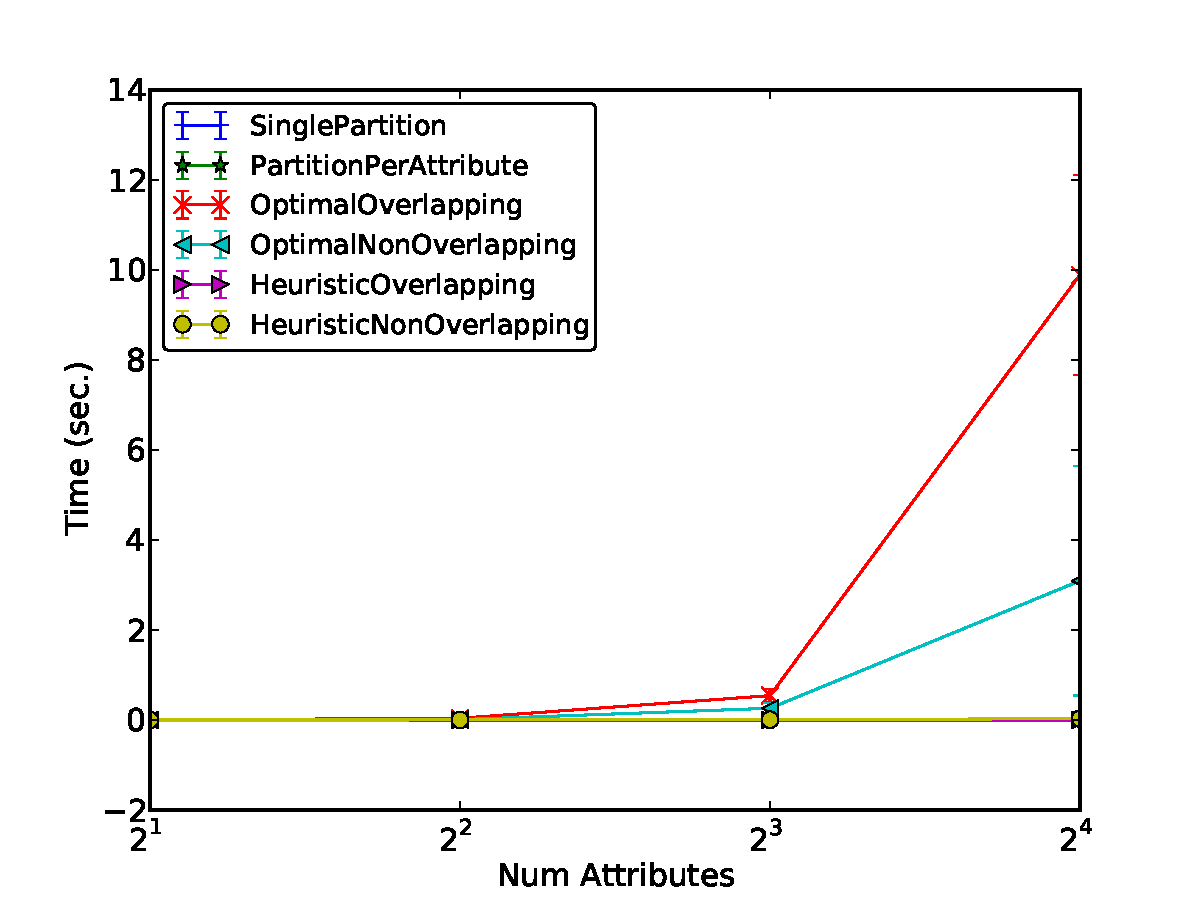
\includegraphics[width=0.33\textwidth]{figures/RunningTimeVsNumAttributes.pdf} &
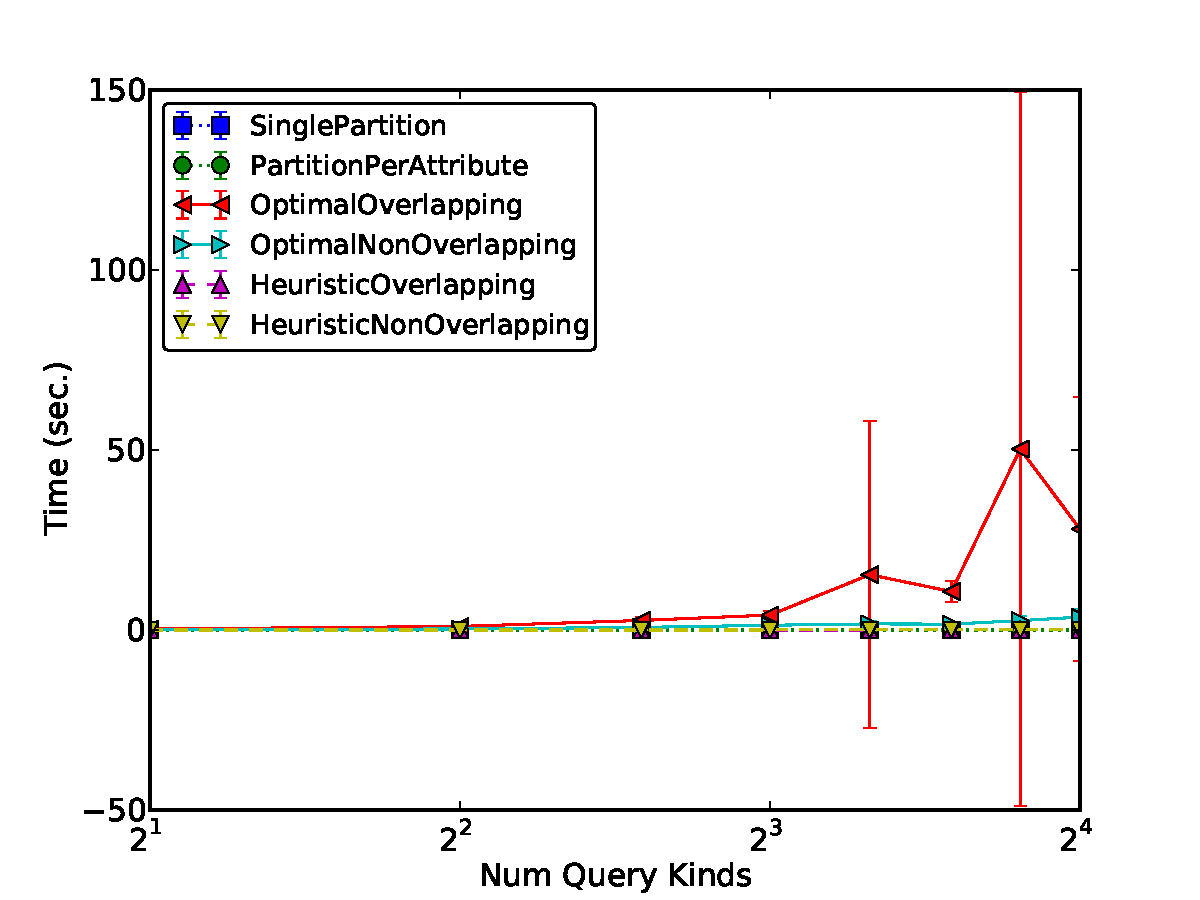
\includegraphics[width=0.33\textwidth]{figures/RunningTimeVsNumQueryKinds.pdf} &
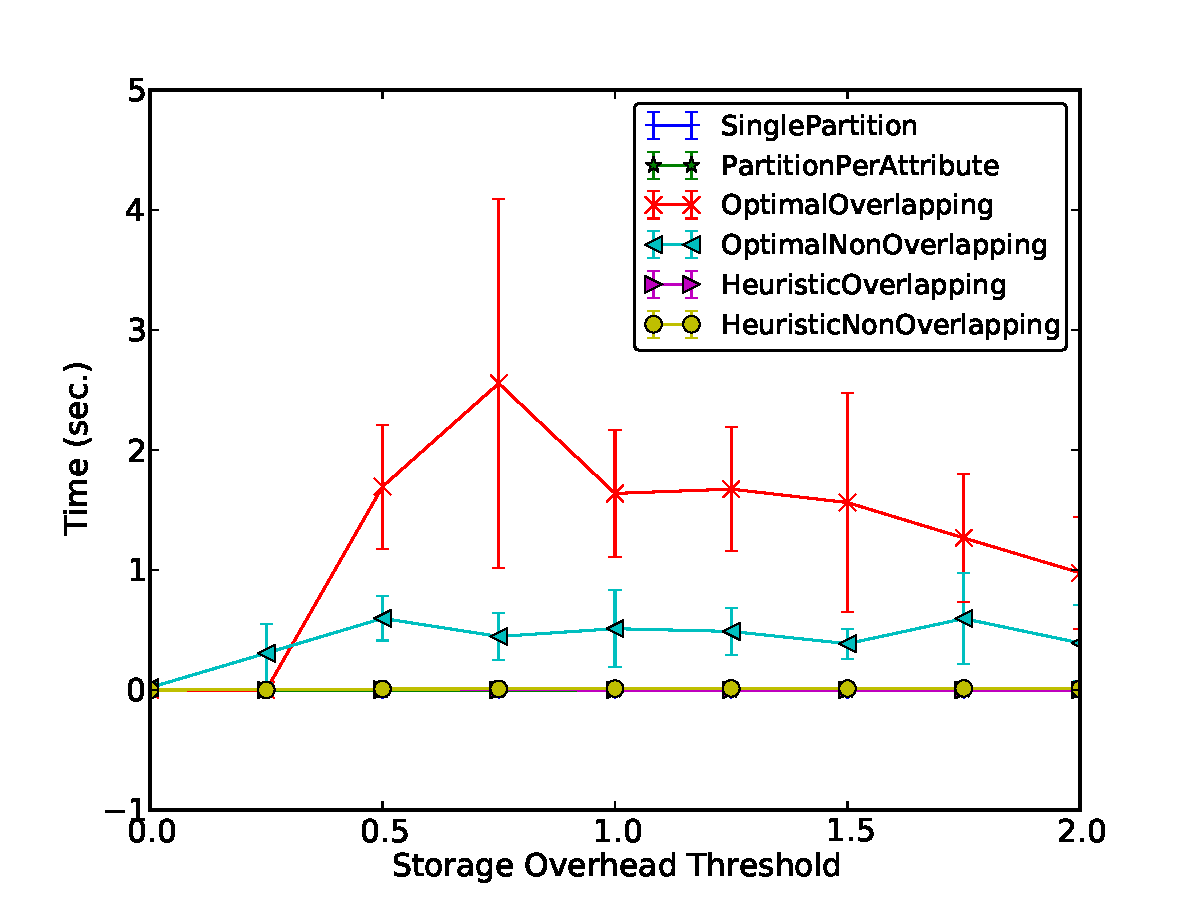
\includegraphics[width=0.33\textwidth]{figures/RunningTimeVsStorageOverheadThreshold.pdf}\\
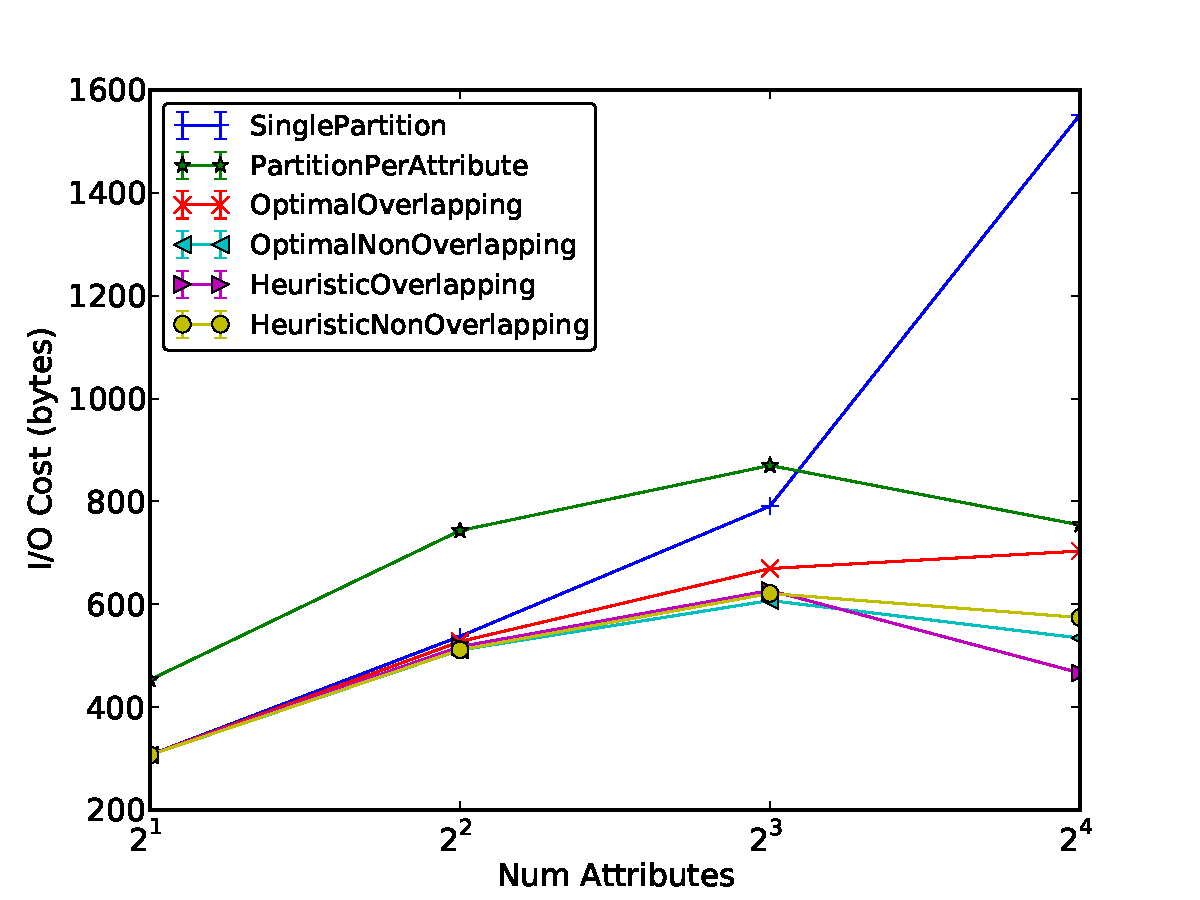
\includegraphics[width=0.33\textwidth]{figures/QueryIOVsNumAttributes.pdf} &
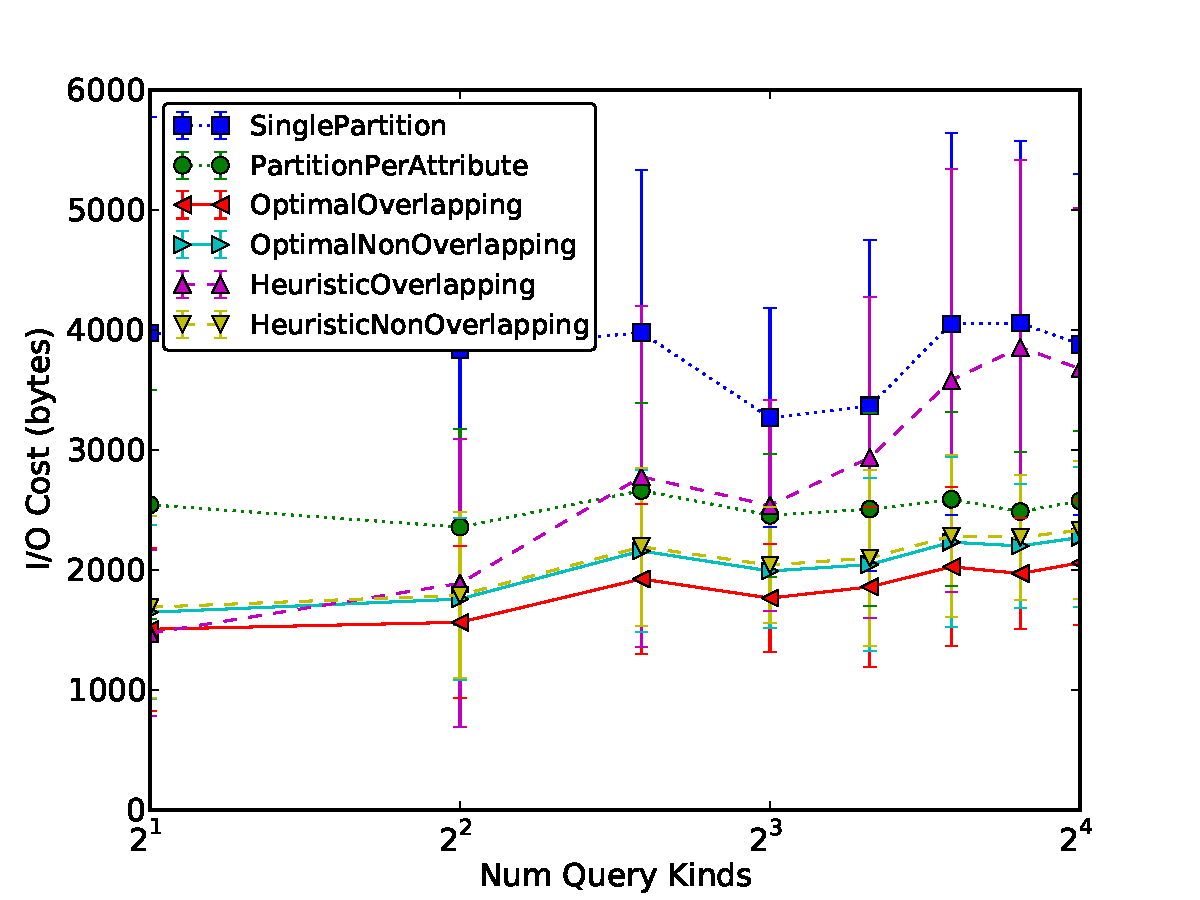
\includegraphics[width=0.33\textwidth]{figures/QueryIOVsNumQueryKinds.pdf} &
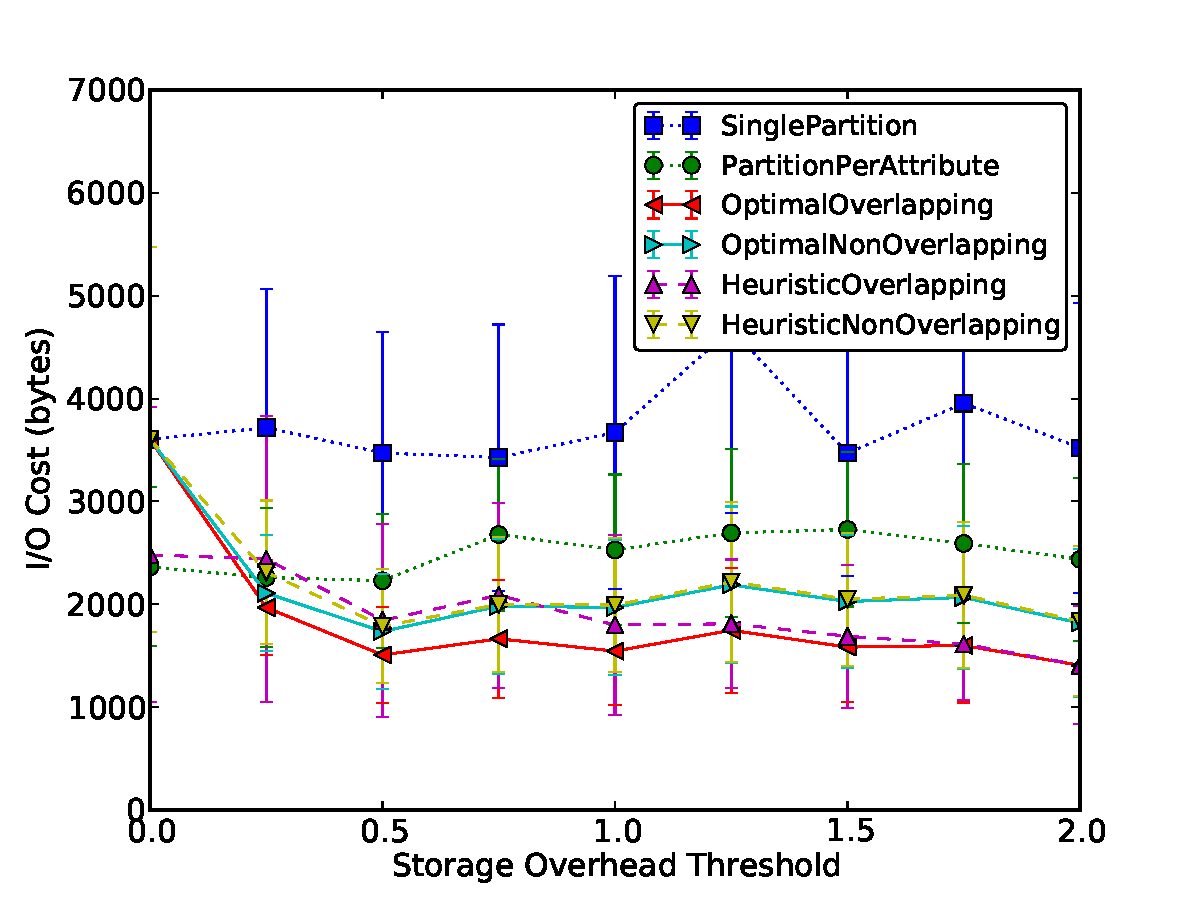
\includegraphics[width=0.33\textwidth]{figures/QueryIOVsStorageOverheadThreshold.pdf}\\
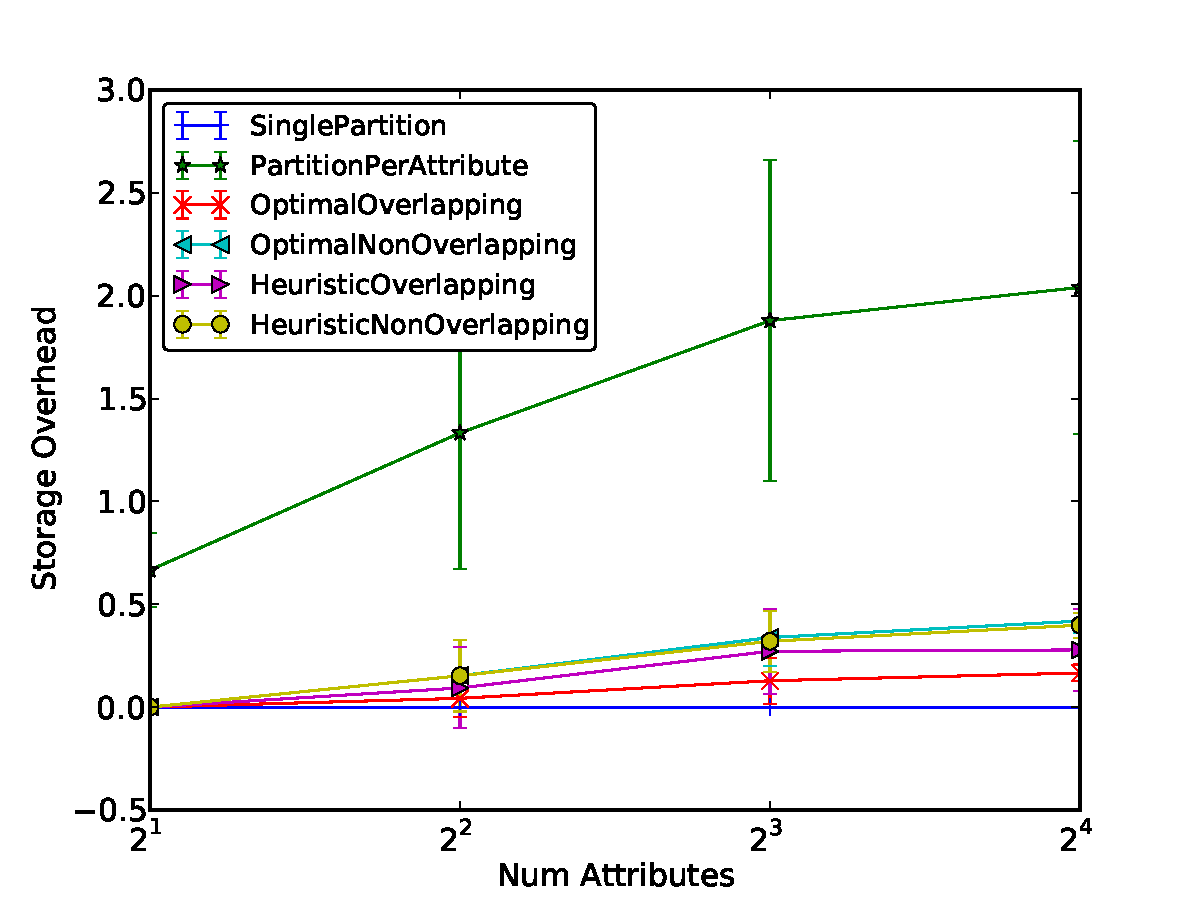
\includegraphics[width=0.33\textwidth]{figures/StorageOverheadVsNumAttributes.pdf} &
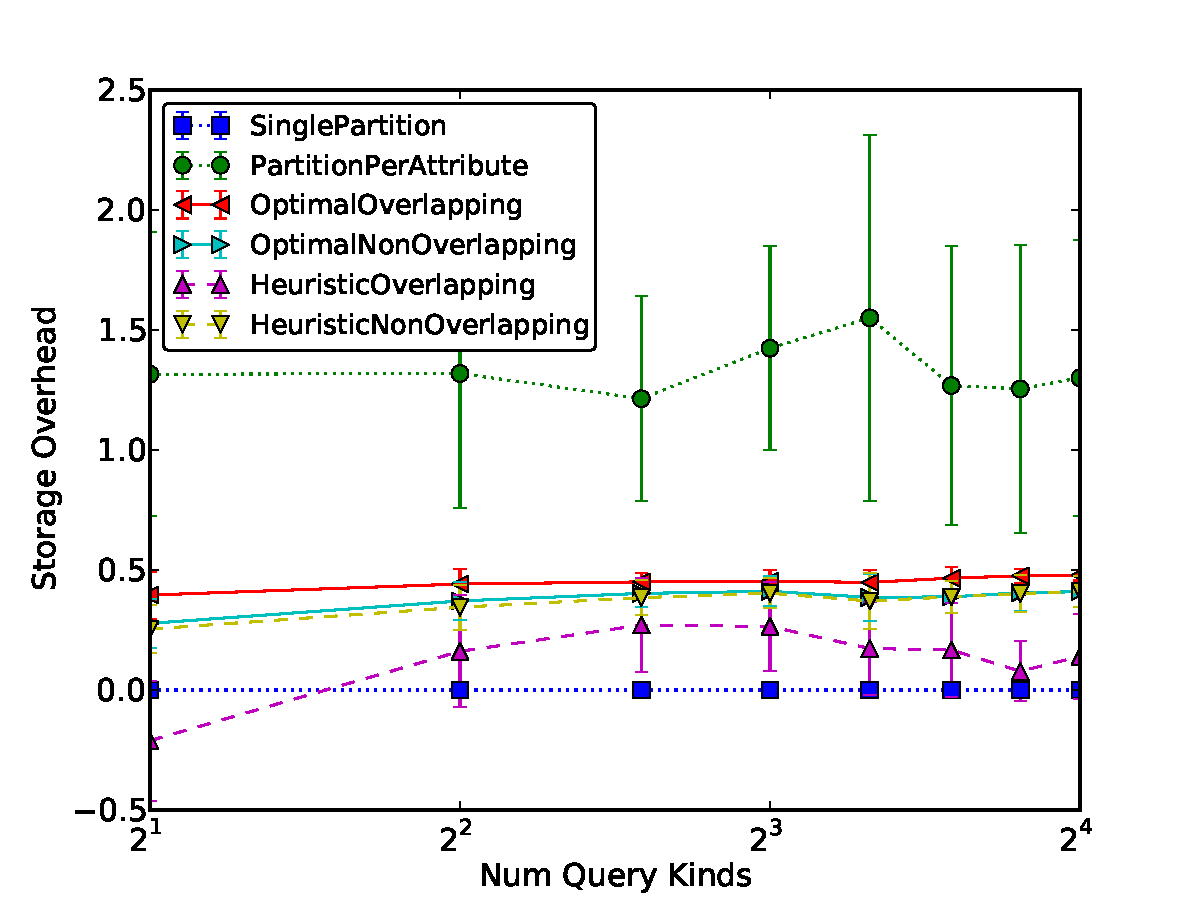
\includegraphics[width=0.33\textwidth]{figures/StorageOverheadVsNumQueryKinds.pdf} &
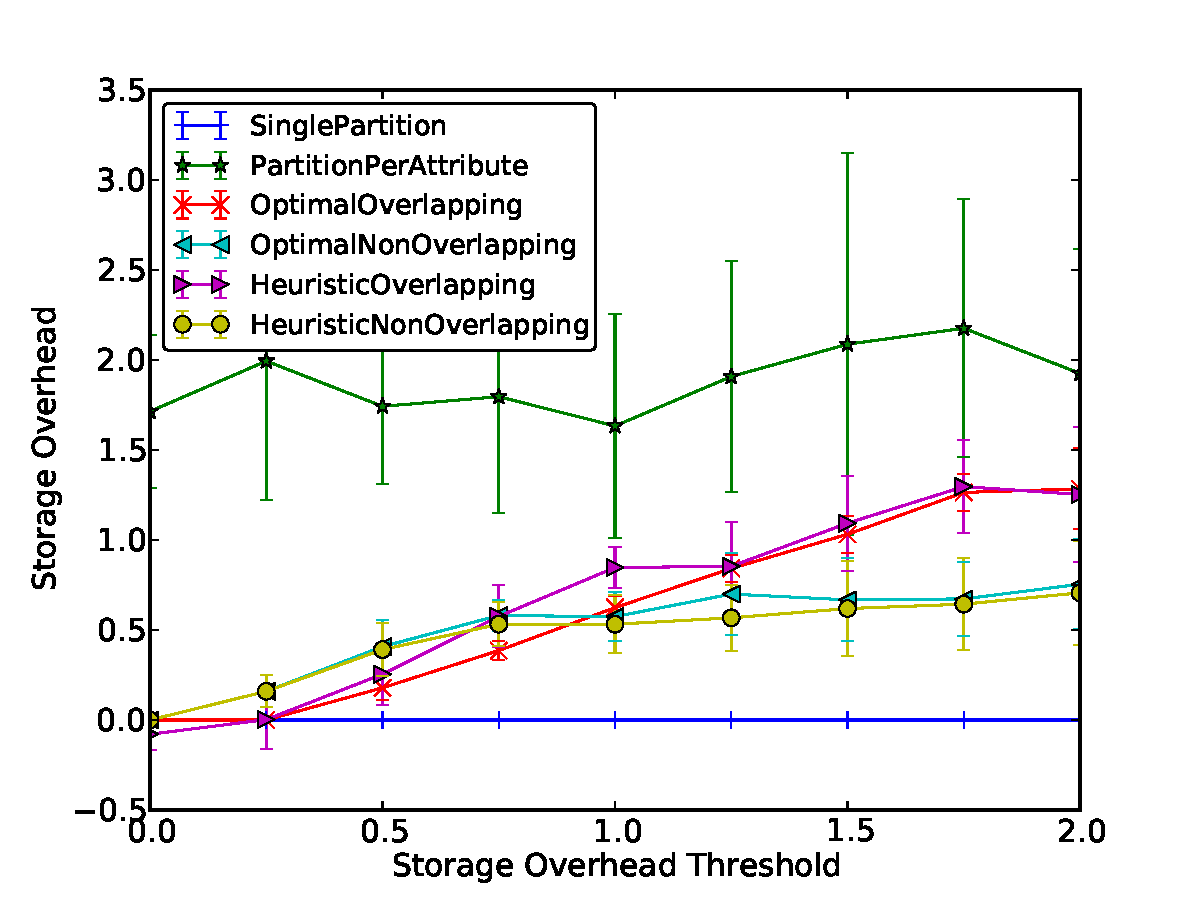
\includegraphics[width=0.33\textwidth]{figures/StorageOverheadVsStorageOverheadThreshold.pdf}\\
(a)Num Attributes & (b) NumQueryKind &
(c) StorageOverheadThreshold \\
\end{tabular}}
 \caption{Running time, QueryIO, and StorageOverhead.}
 \label{fig:results}
 \end{figure*}
